\usetikzlibrary{calc}
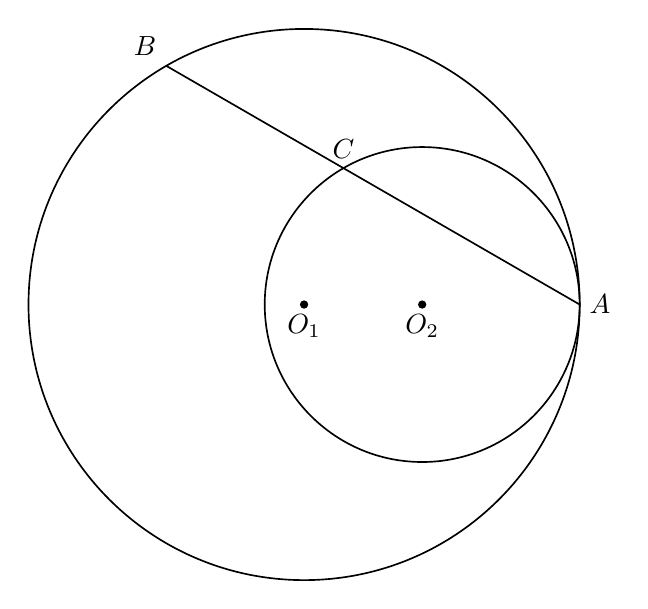
\begin{tikzpicture}[x=1cm,y=1cm,line width=.6pt,font=\normalsize]
\coordinate (O1) at (0,0);
\coordinate (O2) at (1.5,0);
\coordinate (A) at (3.5,0);
\coordinate (B) at (-1.75,3.03109);
\coordinate (C) at (0.5,1.73205);
\draw (O1) circle[radius=3.5cm];
\draw (O2) circle[radius=2cm];
\draw (B)--(A);
\fill (O1) circle (1.5pt);
\fill (O2) circle (1.5pt);
\node[above left] at (B) {$B$};
\node[above] at (C) {$C$};
\node[right] at (A) {$A$};
\node[below] at (O1) {$O_{1}$};
\node[below] at (O2) {$O_{2}$};
\end{tikzpicture}
